\section{Metodologia}

\subsection{Princípio de Arquimedes}
Este experimento é dividido em duas partes. A primeira parte consiste na 
determinação da densidade de um material denominado ``ouro''. Para realização desta
utilizam-se uma jarra com água, uma balança digital e um sólido de dimensões 
significativas. Primeiro, coloca-se a jarra com água sobre a balança digital, 
então o sólido é submerso na água. Por fim, registra-se a força peso indicada na 
balança, este processo pode ser observado na \cref{ouro.png}.

\begin{figure}[H]
    \centering
    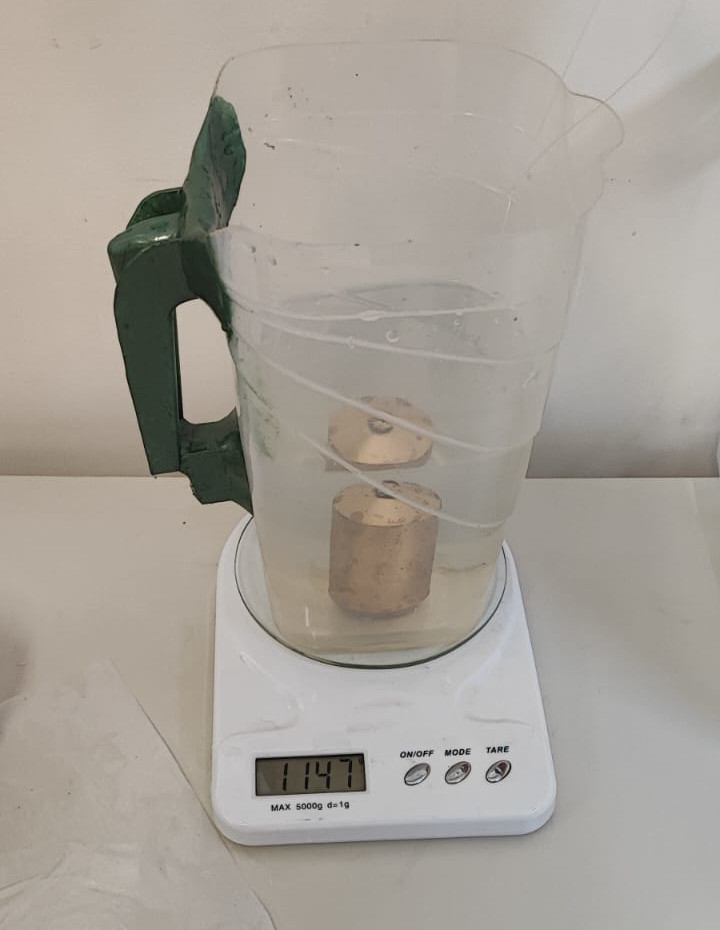
\includegraphics[width=.25\linewidth]{fig/ouro.jpeg}
    \caption{Sólido de ``ouro'' submerso na jarra com água sobre a balança digital}
    \label{ouro.png}
\end{figure}

A segunda parte do experimento objetiva estudar a força de empuxo. Para tanto,
são utilizados dois sólidos de volume igual (\(V_{s1} = V_{s2} = \qty{702}{cm ^2}\))
e massas distintas: (\(m_{s1} = \qty{1337}{g}, m_{s2} = \qty{688}{g}\)), uma balança 
digital, uma jarra preenchida com água suficiente para submergir um sólido de cada vez
sem transbordar e um dinamômetro. O procedimento é realizado como segue: um cilindro 
por vez é pendurado no dinamômetro e, segurando o dinamômetro, submerge-se o cilindro.
Para a coleta de dados deve-se observar a força mensurada no dinamômetro antes e após 
submergir o cilindro. É possível observar a tomada de medidas em um dos cilindros na \cref{arquimedes.png}.
Também deve-se anotar a massa mensurada na balança. É recomendável  utilizar a função ``tara'' da balança digital 
com apenas a jarra com água encima. Caso contrário,
pode-se anotar a diferença de massa.

Em particular, a balança digital utilizada neste trabalho apresenta erro de 
\(\pm \qty{1}{g}\).
\begin{figure}[H]
    \centering
    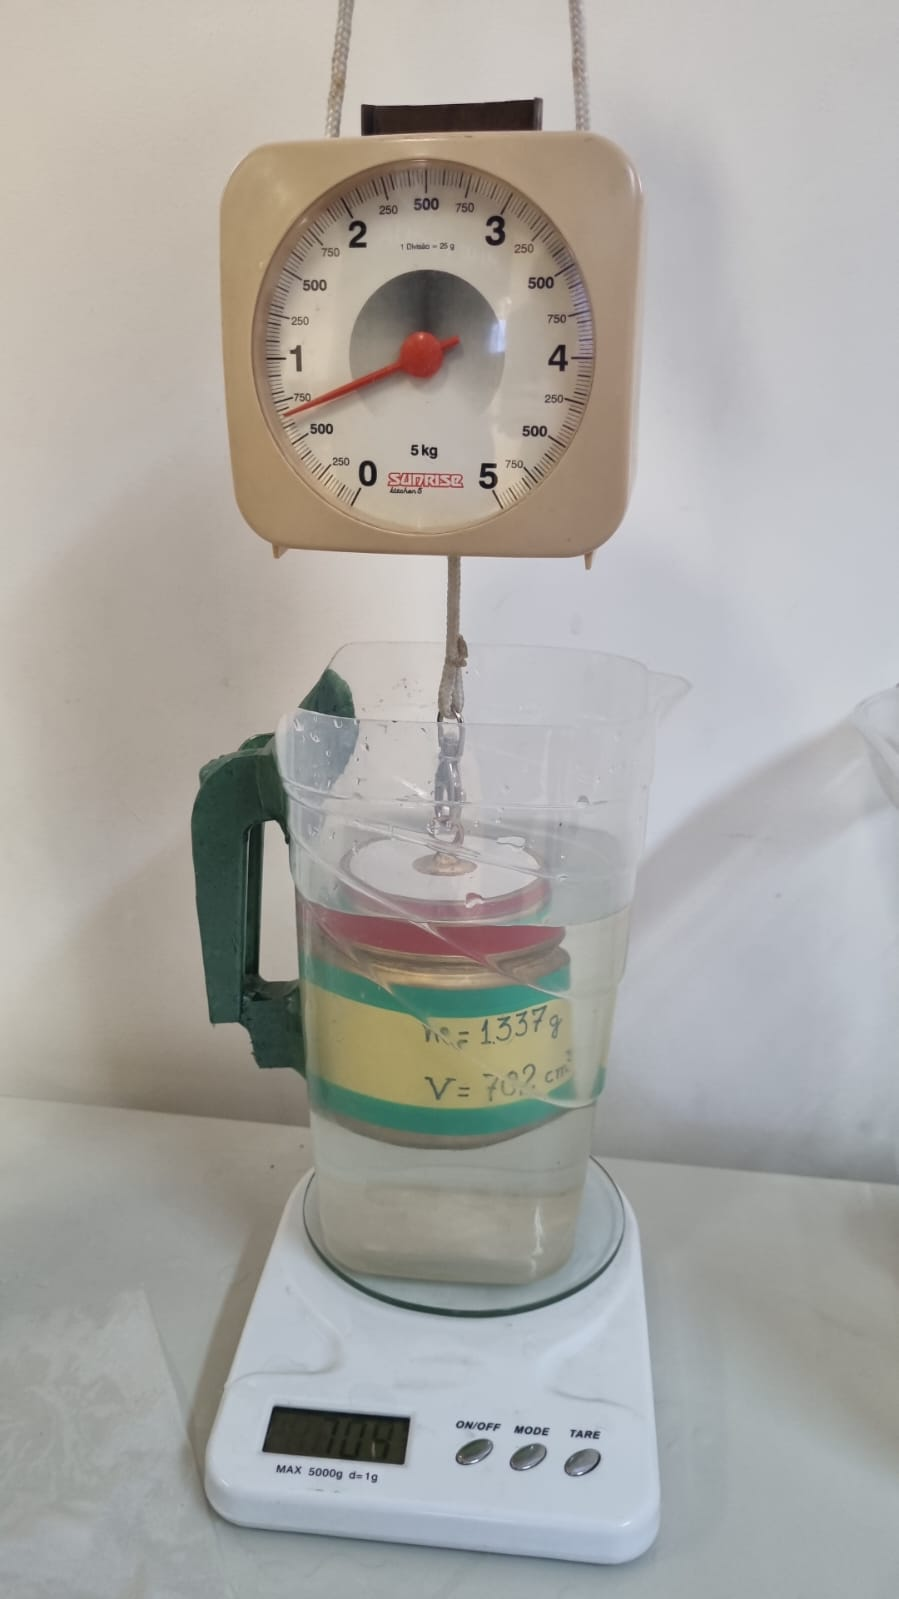
\includegraphics[width=.25\linewidth]{fig/arquimedes.jpeg}
    \caption{Cilindro suspenso em dinamômetro e submerso em água sobre balança digital}
    \label{arquimedes.png}
\end{figure}

\subsection{Balança de empuxo}
Para a demonstração é necessário confeccionar uma balança de empuxo. A balança
de empuxo consiste em um cilindro maior, no qual deve-se encaixar um cilindro
menor de densidade consideravelmente inferior à da água e diâmetro próximo ao
diâmetro do cilindro maior sobre o qual fica preso um prato. É considerado o ponto
de massa zero da balança quando a garrafa está em equilíbrio estático sem nenhum 
objeto estar apoiado sobre o prato. A partir deste ponto, coloca-se uma graduação
de massa pesada de acordo com o nível da água entre os cilindros. O objeto a ser
estudado deve ser apoiado sobre o prato e o nível da água deve ser anotado após
a balança entrar em equilíbrio estático. É possível observar a tomada de uma medida de
massa na \cref{empuxo.png}
\begin{figure}[H]
    \centering
    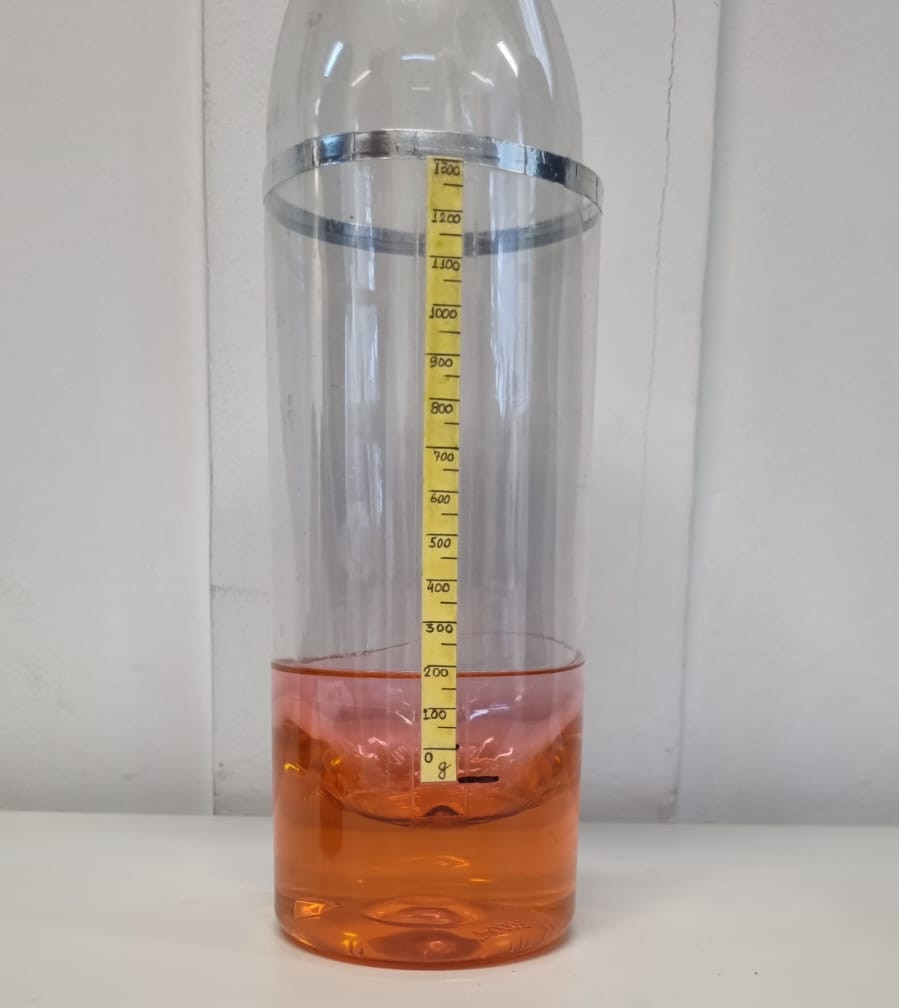
\includegraphics[width=.25\linewidth]{fig/empuxo.jpeg}
    \caption{Medida da massa de um objeto na balança de empuxo}
    \label{empuxo.png}
\end{figure}

\subsection{Gangorra}
Neste experimento é utilizada uma bacia paralelepipédica parcialmente preenchida
com água. A bacia é apoiada sobre um paralelepípedo de comprimento
consideravelmente menor que o comprimento da bacia, de forma que ela possa ser
desequilibrada na presença de torque. No meio da bacia coloca-se uma barreira de
comprimento delgado, porém profundidade próxima de dois terços da profundidade
da própria bacia e altura igual a altura da bacia. A experimentação consiste em
apoiar um pote de desnidade menor que a água de um dos lados da bacia, de
maneira que fique suspenso. Então, uma pedra (ou outro sólido mais denso que a
água) é colocado hora dentro do pote suspenso, hora diretamente na bacia.
Deve-se observar os efeitos de colocar a pedra dentro do pote ou diretamente na
bacia. A bacia apoiada sobre o paralelepípedo é o que chamamos de gangorra. É posssível observar 
a gangorra preenchida com água e com a pedra dentro do pote em equilíbrio na \cref{gangorra.png}.
Por conveniência, doravante, nos referimos ao pote por barco.  
\begin{figure}[H]
    \centering
    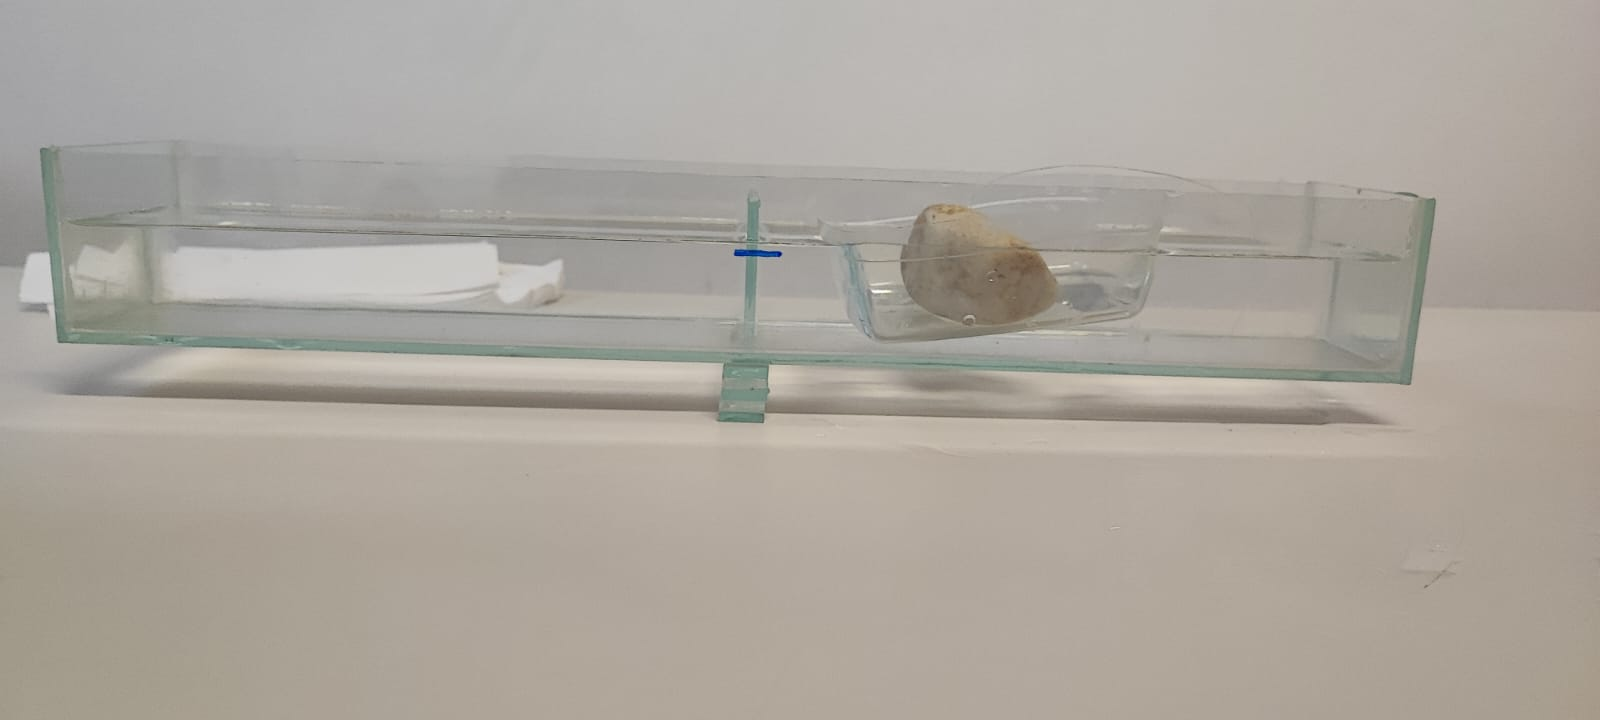
\includegraphics[width=.35\linewidth]{fig/gangorra.jpeg}
    \caption{gangorra em equilíbrio}
    \label{gangorra.png}
\end{figure}

\subsection{Bonecos flutuantes}
Para esta demonstração, colocam-se dois bonecos em uma garrafa tampada quase
completamente preenchida com água. Um dos bonecos tem densidade menor que a água
enquanto o outro é mais denso que a água, doravante serão denominados boneco 
flutuante e boneco não-flutuante, respectivamente. O boneco flutuante deve
ter um gancho que ficará com a concavidade para cima, enquanto o boneco não-flutuante
deve ter um gancho com concavidade para baixo, conforme a \cref{bonecos.png}. Deve-se observar de que
forma, sem abrir a garrafa, é possível fazer ambos os bonecos subirem juntos. 
\begin{figure}[H]
    \centering
    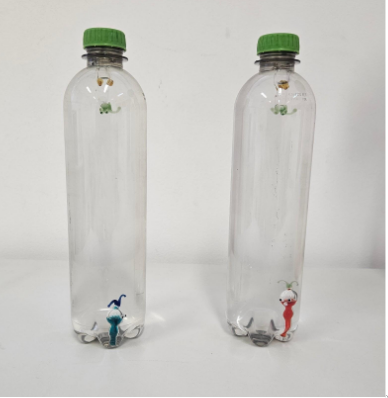
\includegraphics[width=.25\linewidth]{fig/bonecos.png}
    \caption{Duas garrafas com os bonecos flutuante e não-flutuante}
    \label{bonecos.png}
\end{figure}
%TODO: colocar imagens

